\documentclass[conference]{IEEEtran}
\usepackage[T1]{fontenc}
\usepackage{mathptmx}
\usepackage{amsmath}
\usepackage{graphicx}
\usepackage{balance}
\title{A Two-Way Set-Associative Cache with Exact LRU\\Phase I Prototype}
\author{\IEEEauthorblockN{Aaditya Yadav, Gauri Mishra, Bhumi Rastogi, Ansh Sharma, and Anugra}}
\begin{document}
\maketitle
\begin{abstract}
This work implements a 128-byte, two-way set-associative cache in Verilog.
The prototype uses 16 sets of 4-byte lines, exact least-recently-used (LRU)
replacement, and a write-back, write-allocate policy. A blocking controller
coordinates parallel tag comparisons, victim write-back, and refill. A
self-checking testbench passed 15 transactions covering hits, misses,
replacement order, dirty-data persistence, and interface edge cases.
\end{abstract}
\begin{IEEEkeywords}
cache, set associativity, least recently used, write-back, Verilog
\end{IEEEkeywords}

\section{Literature Review}
A direct-mapped cache maps each block to one line. It requires one tag
comparison, but blocks sharing a location can repeatedly displace each
other. A set-associative cache allows several blocks in the same set to
coexist. It needs parallel tag comparisons, way selection, and replacement
state. Hill and Smith analyze how associativity affects miss behavior~\cite{hill}.

LRU evicts the resident line whose last reference is oldest.
Mattson \emph{et al.} describe stack processing for evaluating storage
hierarchy replacement behavior~\cite{mattson}. Tree-based pseudo-LRU
approximates recency in wider sets. One bit tracks exact recency for two
ways. FIFO orders lines by insertion and ignores hits. Random replacement
needs no history of the access order. Workload locality and hardware cost
affect policy choice.

For a blocking cache, average memory access time is
\begin{equation}
T_{\mathrm{AMAT}} = T_{\mathrm{hit}} + r_{\mathrm{miss}} P_{\mathrm{miss}},
\end{equation}
where the miss penalty is the extra time beyond a hit. It includes the
refill time and, for a dirty victim, the preceding write-back time.
Comparative AMAT requires representative traces and a timing model.

\section{Proposed Solution}
\subsection{Datapath}
A 32-bit byte address comprises tag bits [31:6], set bits [5:2], and offset
bits [1:0]. Each aligned 32-bit word spans a line. The index selects two
ways, each storing a tag, data word, valid bit, and dirty bit. Valid bits
qualify parallel tag comparisons. Synchronous reset clears valid and dirty
bits. Figure~\ref{fig:block} shows the main blocks.

\begin{figure}[t]
\centering
\setlength{\unitlength}{0.93pt}
\begin{picture}(244,104)
\put(0,79){\framebox(46,22){CPU}}
\put(77,79){\framebox(88,22){Controller}}
\put(197,79){\framebox(47,22){Memory}}
\put(47,93){\vector(1,0){29}}
\put(76,86){\vector(-1,0){29}}
\put(166,93){\vector(1,0){30}}
\put(196,86){\vector(-1,0){30}}
\put(77,43){\framebox(88,18){Address decoder}}
\put(121,79){\vector(0,-1){17}}
\put(0,5){\framebox(72,20){Tag array}}
\put(84,5){\framebox(74,20){Data array}}
\put(171,5){\framebox(73,20){LRU unit}}
\put(77,52){\line(-1,0){41}}
\put(36,52){\vector(0,-1){27}}
\put(121,43){\vector(0,-1){18}}
\put(165,52){\line(1,0){42}}
\put(207,52){\vector(0,-1){27}}
\end{picture}
\caption{Cache blocks and address-selection paths. Top-level wiring also routes hit, victim, and update signals between the controller and storage blocks.}
\label{fig:block}
\end{figure}

\subsection{Controller and Write Policy}
The controller accepts one request in \textsc{Idle} and latches its
operands. In \textsc{Tag Compare}, a read hit returns the cached word.
A write hit changes the data and sets the dirty bit. An unaligned request
returns an error with no memory command. A dirty victim triggers
\textsc{Writeback}. The victim address combines the victim tag with the
request set and a zero offset. Clean or invalid victims go to \textsc{Refill}.

A rising edge with memory valid and ready completes a command. A write-back
must complete before refill starts. A load installs the returned word as
clean. A store installs the CPU write data as dirty, completing write
allocation. \textsc{Done} emits a one-cycle response before returning to
\textsc{Idle}.

\begin{figure}[t]
\centering
\setlength{\unitlength}{0.93pt}
\begin{picture}(244,111)
\put(0,88){\framebox(50,20){IDLE}}
\put(73,88){\framebox(96,20){TAG COMPARE}}
\put(196,88){\framebox(48,20){DONE}}
\put(50,98){\vector(1,0){23}}
\put(169,98){\vector(1,0){27}}
\put(0,38){\framebox(83,20){WRITEBACK}}
\put(137,38){\framebox(64,20){REFILL}}
\put(105,88){\line(0,-1){13}}
\put(105,75){\line(-1,0){64}}
\put(41,75){\vector(0,-1){17}}
\put(154,88){\vector(0,-1){30}}
\put(83,48){\vector(1,0){54}}
\put(201,48){\line(1,0){20}}
\put(221,48){\vector(0,1){40}}
\put(0,8){\makebox(244,16)[l]{DONE returns to IDLE after the response.}}
\end{picture}
\caption{Controller states. Hits and alignment errors go directly to DONE. Misses refill directly or wait for a dirty write-back.}
\end{figure}

\subsection{Replacement}
An invalid line always takes priority. If both are invalid, way 0 is
chosen first. If both are valid, the stored LRU bit selects the victim.
A hit or completed fill sets only the addressed set's bit to $1-w$,
where $w$ is the accessed way.

\section{Prototype Verification}
Icarus Verilog passed 15 self-checking transactions with nine refills and
one write-back. Addresses \texttt{0x014}, \texttt{0x054}, \texttt{0x094}, and
\texttt{0x0D4} share set 5. Touching the first address before the third fill
preserved it and evicted the second address. Later, a request to
\texttt{0x0D4} evicted dirty \texttt{0x014}. The testbench checked the
write address and payload and verified that a later read refilled the
updated value. It also checked write allocation, set isolation, unaligned
access, and reset. The behavioral memory models 4 KiB with a fixed delay.

\begin{figure}[!t]
\centering
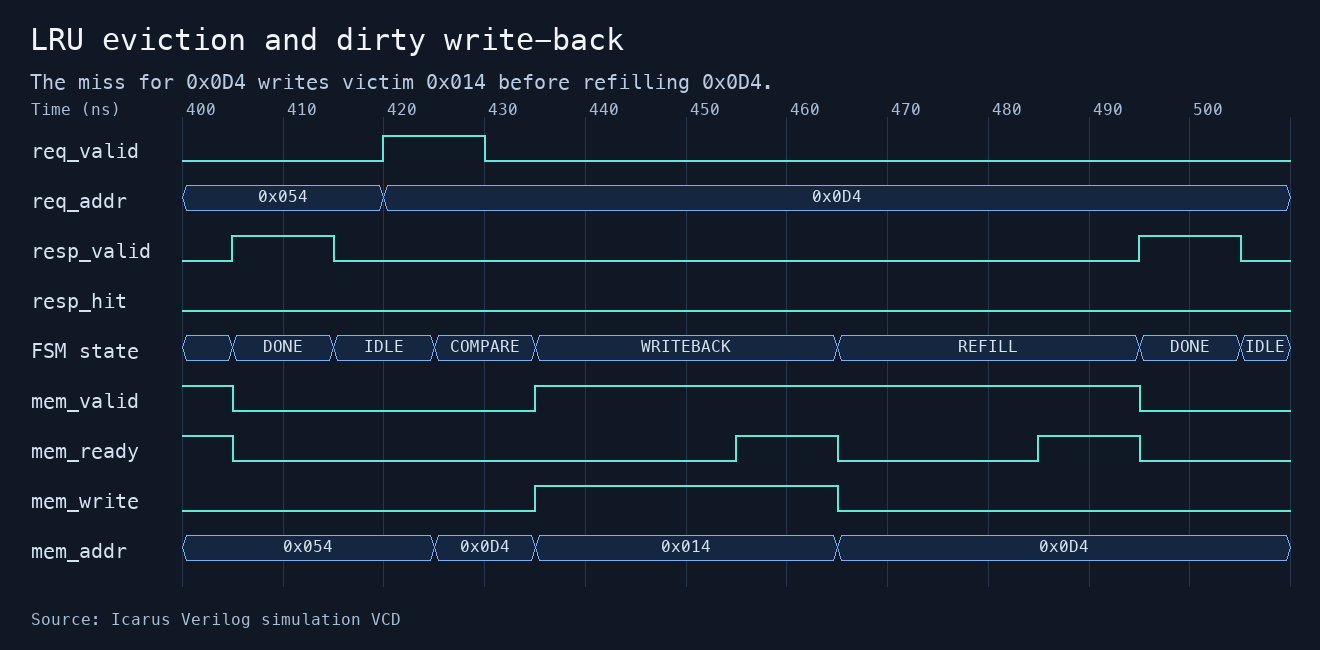
\includegraphics[width=\columnwidth]{../sim/lru-dirty-eviction.png}
\caption{Simulation trace for the dirty LRU victim. The controller writes 0x014 before it refills 0x0D4. The full-resolution trace is in the simulation directory.}
\end{figure}

\balance
\section{Individual Contributions}
The team assignments for review and repository integration are:
\begin{itemize}
\item Aaditya Yadav --- behavioral memory, tests, and waveforms.
\item Gauri Mishra --- controller FSM, write policy, and integration.
\item Bhumi Rastogi --- tag and data arrays and address decoding.
\item Ansh Sharma --- LRU state updates and victim selection.
\item Anugra --- report, diagrams, and README.
\end{itemize}

\section{Phase II Plan}
Replay sequential, strided, and random traces against this cache and an
equal-capacity direct-mapped baseline. Record misses, write-backs, and
response latency. An optional FPGA build can measure resource use and
achievable clock frequency.

\begin{thebibliography}{2}
\bibitem{hill}
M. D. Hill and A. J. Smith, \textquotedblleft Evaluating associativity in CPU
caches,\textquotedblright{} \emph{IEEE Trans. Comput.}, vol. 38, no. 12,
pp. 1612--1630, Dec. 1989, doi: 10.1109/12.40842.
\bibitem{mattson}
R. L. Mattson, J. Gecsei, D. R. Slutz, and I. L. Traiger,
\textquotedblleft Evaluation techniques for storage hierarchies,\textquotedblright{}
\emph{IBM Syst. J.}, vol. 9, no. 2, pp. 78--117, 1970,
doi: 10.1147/sj.92.0078.
\end{thebibliography}
\end{document}
